\subsection{Metrics for operator}
PIVOT supports the network operator in its routine operations, providing a series of statistical metrics that illustrate the current state of the administered network.

\subsubsection{Number of Joins (NoJ)}
The Number of Joins (NoJ) represents the overall \textit{Join-request} messages intercepted and registered by PIVOT over the time. Generally, in LoRaWAN there is a \textit{peak} of Join-requests only in the starting phase when the operator registers and activates all the devices that will operate in the network. All Join-requests following this peak denote the insertion of new devices or the reconnection of old ones, two uncommon events. A too high value of NoJ might indicate the malfunction of one or more devices that are disconnecting and reconnecting continuously from the network. As demonstrated, sending a Join-request message could involve the expose the addresses of the device to unauthorized parties, then operator should avoid that the EDs send too many messages of this type.

\vspace{3mm}
\begin{figure}[H]
    \centering
    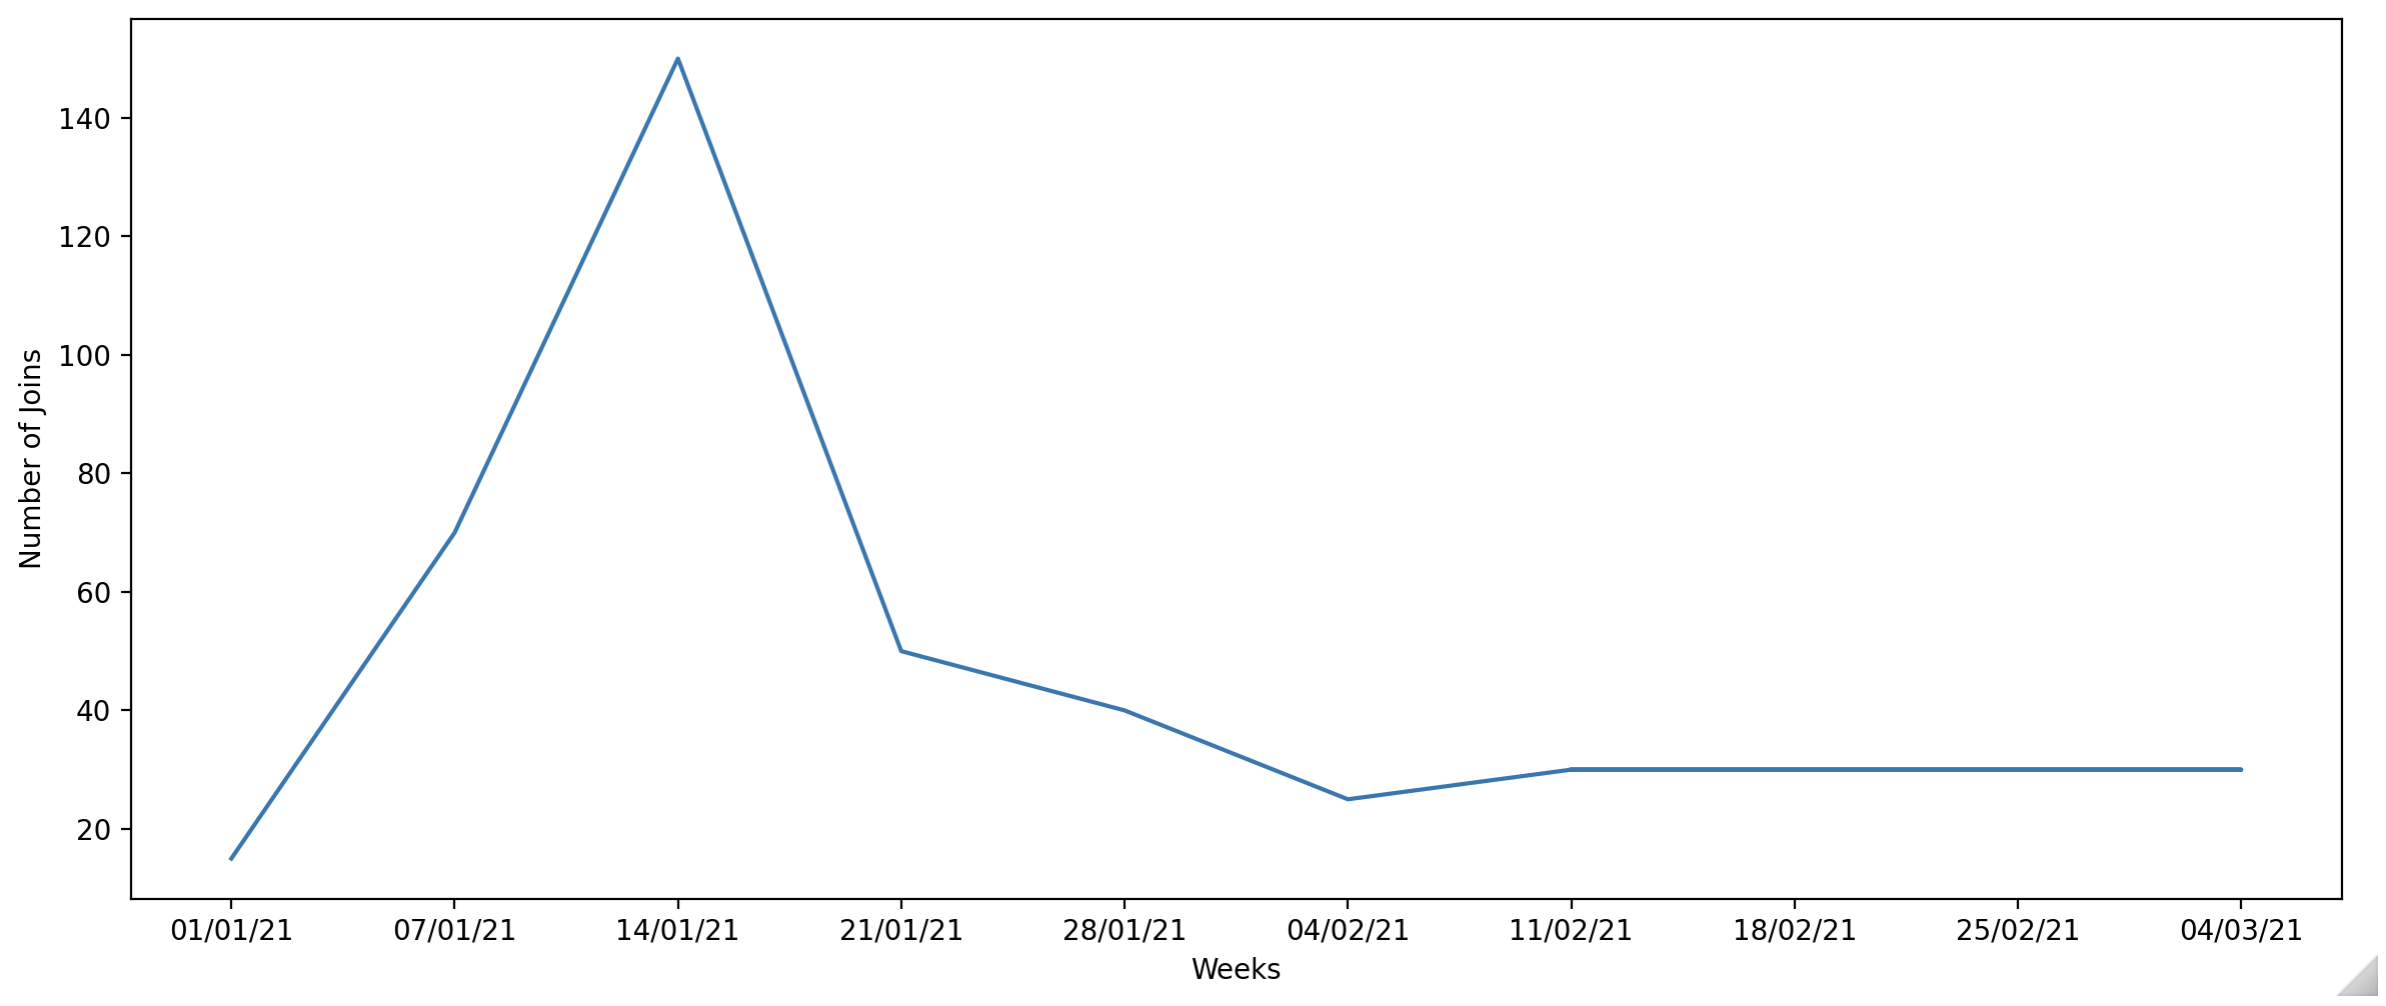
\includegraphics[width=0.7\linewidth]{images/pivot/NoJ.png}
    \caption{This plot reports an example of NoJ/weeks of a LoRaWAN network without anomaly devices. There is a peak only in the initial phase.}
    \label{fig:noj}
\end{figure}
\vspace{3mm}

\subsubsection{Number of Detected Devices (NoDD)}
The Number of Detected Devices (NoDD) describes the current amount of devices classified by PIVOT as vulnerable. These EDs, that re-joined the network at least once, have a too predictable pattern that could disclose their sensible characteristics, such as the identifiers, to external eavesdroppers. NoDD is updated each time PIVOT triggers the alert to the operator. This metric depends on the \textit{accuracy} of the detection algorithm of PIVOT, which may \textit{misclassify} some devices or miss capturing all vulnerable ones.

\subsubsection{Number of Unique Devices (NoUD)}
The Number of Unique Devices (NoUD) is the number of ED registered by PIVOT. These devices have sent at least one message to the server, exposing their DevAdress. NoUD does \textit{not} represent the total amount of devices of the network but only those that have transmitted packets since PIVOT was turned on. NoUD indicates the number of \textit{currently active} devices.

\subsubsection{Percentage of Detected Devices (PoDD)}
The Percentage of Detected Devices (PoDD) is a value in the range [0, 1] and represents the ratio between \textit{NoDD} and \textit{NoUD}. It provides a clear view of the network, showing exactly how many devices are vulnerable among all those present. Since it is not unusual for LoRa devices to generate periodic traffic, the PoDD value is generally always greater than zero. Using this metric, the operator can establish the \textit{maximum} permissible percentage of exposed devices, according to the dimension of the network. For example, in the case of environments made by a consistent number of devices, the management becomes more complex, and it is almost impossible to handle all the devices exposed. In this case, the goal could be to reduce the value of \textit{PoDD} whenever possible.